\documentclass[10pt,a4paper]{article}
\usepackage[latin1]{inputenc}
\usepackage{amsmath}
\usepackage{amsfonts}
\usepackage{amssymb}
\usepackage{graphicx}


\author{Grupe 02}
\title{PflichtenHeft}
\begin{document}
% Title Page
\maketitle
% Inhaltsverzeichniss
\tableofcontents
%------------------------------------------------
% Zielbestimmung
%------------------------------------------------
\section{Zielbestimmung}
	\subsection{Musskriterien}
	\begin{itemize}
		\item Webanwendung
		\begin{itemize}
			\item Startseite
			\item am Corporate Design der Universitaet und Klik-Webseite orientiert
			\item ohne Anmeldung ist nur die Startseite und die Aktivitaetsliste einsehbar
			\item Registrierung fuer Teilnehmer mit Benutzername, Email-Adresse und Dienststelle/Studiengang erfordert.
			\item Jeder Teilnehmer und jedes Team hat ein oeffentlich einsehbares Profil (Punkte, Aktivitaeten, Foto,...) %TODO
			\item Teilnehmer sammeln Punkte, und koennen diese einsehn
			\item Teilnehmer koennen sich zu Teams zusammenschliessen um gemeinsam Punkte zusammeln, in diese kann eingeladen werden.
			\item Teilnehmer koennen nur in einem Team Mitglied sein
			\item Teilnehmer koennen Energiesparvorschlaege einreichen
			\item Teilnehmer koennen Aktivitaeten auswaehlen und erledigen
			\item Aktivitaeten haben einen Zeitramen, Heufigkeit, Kategorie und Punkte
			\item Aktivitaeten muessen nach Auswahl bestaetigt werden
			\item Es gibt Challenges die Zeitlich begrenzt sind
			\item An Challenges nimmt jeder automatisch teil
			
			\item Es gibt eine Uebersich ueber alle Energiesparvorschlaege
			\item Energiesparvorschlaege koennen kommentiert werden
			\item Energiesparvorschlaege koennen bewertet werden
			\item Es gibt eine Uebersicht ueber alle Teilnehmer und alle Teams (sortiert nach Name / Punkten) %TODO
			\item Grafische annonymisierte Statistiken:
			\begin{itemize}
				\item Besucherzahl
				\item gesammelte Punkte
				\item erledigte Aktivitaeten
				\item beliebteste Aktivitaeten
			\end{itemize}
		\end{itemize}
		% ----------------------------------------------------------------
		\item Android-App
		\begin{itemize}
			\item Einmaliges login nach registrierung auf der Webseite
			\item Profilseiten sind einsehbar
			\item Ranking von Teilnehmern und Teams einsehbar
			\item Uebersicht aller Aktivitaeten
			\item Aktivitaeten auswaehlen und erledigen
			\item Liste der ausgewaehlten Aktiviaeten
			\item Suchfunktion fuer Teilnehmer, Teams und Aktivitaeten
			
		\end{itemize}
		% ----------------------------------------------------------------
		\item Admin Bereich
		\begin{itemize}
			\item Challenges erstellen
			\item Aktivitaeten erstellen und bearbeiten
			\item Energiesparvorschlaege annehmen
			\item Emails an alle Teilnehmer
			\item Teilnehmer und Teams sperren.
		\end{itemize}
	\end{itemize}
	\subsection{Sollkriterien}
	\begin{itemize}
			\item Profilbild fuer Teilnehmer und Gruppen
			\item Individueller Gruppen Vorschlag nach Registrierung
			\item Admin kann Teilnehmer und Teams reaktivieren und loeschen
			\item Admin kann Teams und Teilnehmer verwarnen
			\item Challenges in App implementiert
			\item Einstellbare Benachrichtigungen fuer App, Browser und Emails
		\end{itemize}
	\subsection{Kannkriterien}
	\begin{itemize}
			\item Profile lassen personalisieren
			\item Admin kann Emails an Einzelteilnehmer und Gruppen senden.
			\item Benutzer wechlsen bei der App
	\end{itemize}
	\subsection{Differentierungskriterien}
	\begin{itemize}
		\item keine direkte Kommunikation unter den Teilnehmern
		\item keine Popups in App und Browser, statt dessen Benachrichitungen 
	\end{itemize}

%------------------------------------------------
% Produkteinsatz
%------------------------------------------------
\section{Produkteinsatz}
\subsection{Answendungsbereich}
\subsection{Zielgruppe}
\subsection{Betriebsbedingungen}

%------------------------------------------------
% Produktumgebung
%------------------------------------------------
\section{Produktumgebung}
\subsection{Software}
\subsection{Hardware}
\subsection{Orgware}

%------------------------------------------------
% Produktuebersicht
%------------------------------------------------
\section{Produkt\"ubersicht}

%------------------------------------------------
% Akteure
%------------------------------------------------
\section{Akteure}

%------------------------------------------------
% Produktfunktion
%------------------------------------------------
\section{Produktfunktion}
\subsection{Webseite}
\begin{figure}[h]
	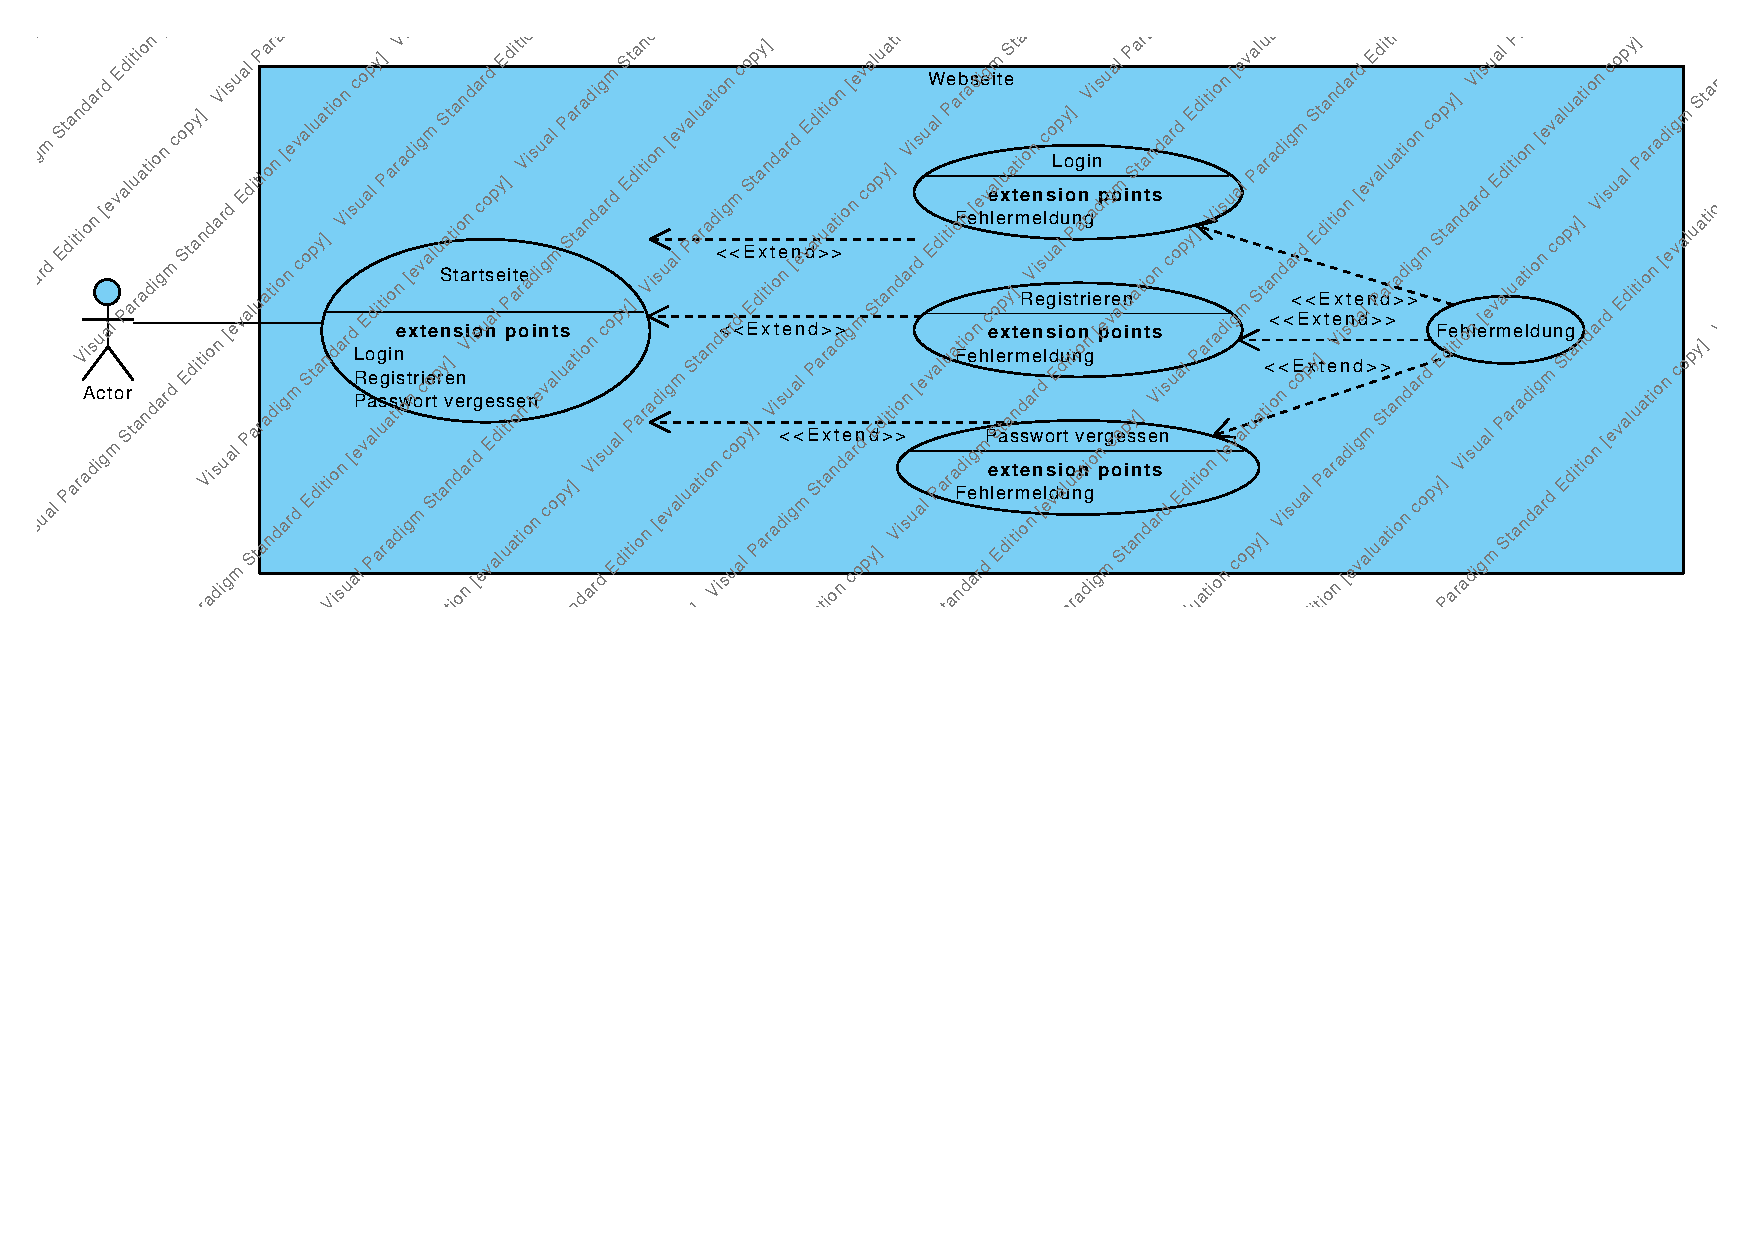
\includegraphics[width=\linewidth,]{gfx/webseite/startseite.pdf}	
\end{figure}
	\subsubsection{Startseite}
	\begin{tabular}{|l|p{.5\linewidth}|}
	\hline Use Case Nummer & 1.1 \\ 
	\hline Use Case Name & Startseite \\ 
	\hline Initiirender Akteur & Benutzer \\
	\hline Weitere Akteure &  \\
	\hline Kurzbeschreibung & der Benutzer ruft die Startseite im Browser auf und hat die M\"oglichkeit sich zu registrieren, einzuloggen und das Passwort neu anzufordern \\
	\hline Vorbedingung & nicht eingeloggt \\
	\hline Nachbedingung &  \\
	\hline \multicolumn{2}{|c|}{Funktionalitaet des UseCases}\\
	\hline Ablauf & Bentuzer ruft die Webseite auf \\
	\hline Alternativen &  \\
	\hline Ausnahmen &  \\
	\hline Benuzte Use Cases &  \\
	\hline \multicolumn{2}{|c|}{Weitere Inforamtionen} \\
	\hline Spezielle Anforderungen &  \\
	\hline Annahmen &  \\
	\hline
	\end{tabular} 
	\subsubsection{Login}
		\begin{tabular}{|l|p{.5\linewidth}|}
		\hline Use Case Nummer & 1.1.1 \\ 
		\hline Use Case Name & Login \\ 
		\hline Initiirender Akteur & Benutzer \\
		\hline Weitere Akteure & Admin \\
		\hline Kurzbeschreibung & Mit dem Login stehen die eigentlichen Funktionen im Browser zur Verf\"ugung \\
		\hline Vorbedingung & Benutzer ist registriert und nicht nicht eingeloggt \\
		\hline Nachbedingung & Benutzer ist eingeloggt \\
		\hline \multicolumn{2}{|c|}{Funktionalitaet des UseCases}\\
		\hline Ablauf & \begin{itemize}
			\item Der Benutzer gibt Email-Adresse und Passwort ein
			\item Der Benutzer klickt den Login Button
		\end{itemize} \\
		\hline Alternativen &  \\
		\hline Ausnahmen & \begin{itemize}
			\item Das Passwort ist falsch, es wird eine Fehlermeldung angezeigt und die Option Passwort vergessen angeboten
			\item Die Email-adresse ist noch nicht registriert, es wird eine Fehlermedldung angezeigt, und die Registrierung angeboten
		\end{itemize} \\
		\hline Benuzte Use Cases &  \\
		\hline \multicolumn{2}{|c|}{Weitere Inforamtionen} \\
		\hline Spezielle Anforderungen &  \\
		\hline Annahmen &  \\
		\hline
		\end{tabular}
			 
	\subsubsection{Registrieren}
		\begin{tabular}{|l|p{.5\linewidth}|}
		\hline Use Case Nummer & 1.1.2 \\ 
		\hline Use Case Name & Registrieren \\ 
		\hline Initiirender Akteur & Benutzer \\
		\hline Weitere Akteure &  \\
		\hline Kurzbeschreibung & Ein neuer Benutzer kann sich mit seiner Email-Adresse anmelden \\
		\hline Vorbedingung & Benutzer hat auf Registrieren geklickt \\
		\hline Nachbedingung & Benutzer ist eingeloggt \\
		\hline \multicolumn{2}{|c|}{Funktionalitaet des UseCases}\\
		\hline Ablauf & \begin{itemize}
			\item Benutzer gibt Email-Adresse und Passwort ein
			\item Benutzer w\"ahlt fakult\"at
			\item Benutzer klickt "jetzt mitmachen"
		\end{itemize} \\
		\hline Alternativen &  \\
		\hline Ausnahmen & \begin{itemize}
			\item Email-adresse ist schon vergeben, es wird eine Fehlermeldung angezeigt
			\item das Passwort ist zu kurz, es wird eine Fehlermeldung angezeit
			\item Keine Fakult\"at gewahlt, es wir eine Fehlermeldung angezeigt
		\end{itemize} \\
		\hline Benuzte Use Cases &  \\
		\hline \multicolumn{2}{|c|}{Weitere Inforamtionen} \\
		\hline Spezielle Anforderungen &  \\
		\hline Annahmen &  \\
		\hline
		\end{tabular} 
		
	\subsubsection{Passwort vergessen}
		\begin{tabular}{|l|p{.5\linewidth}|}
		\hline Use Case Nummer & 1.1.3 \\ 
		\hline Use Case Name & Passwort vergessen \\ 
		\hline Initiirender Akteur & Benutzer \\
		\hline Weitere Akteure &  \\
		\hline Kurzbeschreibung & Ein Benutzer hat die M\"oglichkeit sein Passwort neu anzufordern \\
		\hline Vorbedingung & Benutzer ist nicht eingeloggt \\
		\hline Nachbedingung & Benutzer hat eine Email bekommen \\
		\hline \multicolumn{2}{|c|}{Funktionalitaet des UseCases}\\
		\hline Ablauf & \begin{itemize}
			\item Benutzer gibt seine Email-Adresse an
			\item Benutzer klickt auf "jetzt Passwort anfordern"
		\end{itemize} \\
		\hline Alternativen &  \\
		\hline Ausnahmen & Email-Adresse ist nicht registriert, es wird eine Fehlermeldung angezeigt \\
		\hline Benuzte Use Cases &  \\
		\hline \multicolumn{2}{|c|}{Weitere Inforamtionen} \\
		\hline Spezielle Anforderungen &  \\
		\hline Annahmen &  \\
		\hline
		\end{tabular}
	\subsubsection{Fehlermeldung}
		\begin{tabular}{|l|p{.5\linewidth}|}
		\hline Use Case Nummer & 1.1.4 \\ 
		\hline Use Case Name & Fehlermeldung \\ 
		\hline Initiirender Akteur & Benutzer \\
		\hline Weitere Akteure &  \\
		\hline Kurzbeschreibung & Es wird dem Benutzer eine Fehlermeldung angezeigt und beleibt auf der aktuellen Seite \\
		\hline Vorbedingung &  \\
		\hline Nachbedingung & Fehlermeldung wir angezeigt \\
		\hline \multicolumn{2}{|c|}{Funktionalitaet des UseCases}\\
		\hline Ablauf & Fehlermeldung wird in die Aktuelle Seite eingebettet \\
		\hline Alternativen &  \\
		\hline Ausnahmen &  \\
		\hline Benuzte Use Cases &  \\
		\hline \multicolumn{2}{|c|}{Weitere Inforamtionen} \\
		\hline Spezielle Anforderungen &  \\
		\hline Annahmen &  \\
		\hline
		\end{tabular} 
	 
% MUSTER 
	\subsubsection{Aktivit\"aten ansehen}
	\begin{tabular}{|l|p{.5\linewidth}|}
	\hline Use Case Nummer & 1.3.1 \\ 
	\hline Use Case Name & Aktivit\"aten ansehen \\ 
	\hline Initiierender Akteur & Benutzer \\
	\hline Weitere Akteure & Admin \\
	\hline Kurzbeschreibung & Der Benutzer kann die auf der Seite dargestellte Liste von verf\"ugbaren Aktivit\"aten einsehen \\
	\hline Vorbedingung & Die Aktivit\"atenseite ist im Browser aufgerufen \\
	\hline Nachbedingung & Die Aktivit\"atenseite ist im Browser aufgerufen \\
	\hline \multicolumn{2}{|c|}{Funktionalitaet des UseCases}\\
	\hline Ablauf & 1. Der Benutzer sieht die Liste der Aktivit\"aten an \\
	\hline Alternativen & - \\
	\hline Ausnahmen & Die Aktivit\"atenliste ist nicht verf\"ugbar \\
	\hline Benutzte Use Cases & - \\
	\hline \multicolumn{2}{|c|}{Weitere Inforamtionen} \\
	\hline Spezielle Anforderungen & - \\
	\hline Annahmen & - \\
	\hline
	\end{tabular} 
	
	\subsubsection{Aktivit\"aten ausw\"ahlen}
	\begin{tabular}{|l|p{.5\linewidth}|}
	\hline Use Case Nummer & 1.3.2 \\ 
	\hline Use Case Name & Aktivit\"aten ausw\"ahlen \\ 
	\hline Initiierender Akteur & Benutzer \\
	\hline Weitere Akteure & Admin \\
	\hline Kurzbeschreibung & Der Benutzer kann eine oder mehrere der verf\"ugbaren Aktivit\"aten ausw\"ahlen \\
	\hline Vorbedingung & Die Aktivit\"atenseite ist im Browser aufgerufen und die Liste von Aktivit\"aten wird angezeigt \\
	\hline Nachbedingung & Die Aktivit\"atenliste wird angezeigt, die ausgew\"ahlten Aktivit\"aten sind speziell hervorgehoben \\
	\hline \multicolumn{2}{|c|}{Funktionalitaet des UseCases}\\
	\hline Ablauf & \begin{itemize}
			\item 1. Benutzer w\"ahlt eine oder mehrere Aktivit\"aten aus
			\item 2. Die ausgew\"ahlten Aktivit\"aten werden als ausgew\"ahlt hervorgehoben
		\end{itemize} \\
	\hline Alternativen & - \\
	\hline Ausnahmen & Die Aktivit\"atenliste ist nicht verf\"ugbar \\
	\hline Benutzte Use Cases & 1.3.1 Aktivit\"aten ansehen \\
	\hline \multicolumn{2}{|c|}{Weitere Inforamtionen} \\
	\hline Spezielle Anforderungen & - \\
	\hline Annahmen & Der Benutzer w\"ahlt nur Aktivit\"aten aus, die noch nicht ausgew\"ahlt sind \\
	\hline
	\end{tabular}
	
	\subsubsection{Aktivit\"aten als erledigt abhaken}
	\begin{tabular}{|l|p{.5\linewidth}|}
	\hline Use Case Nummer & 1.3.2.1 \\ 
	\hline Use Case Name & Aktivit\"aten als erledigt abhaken \\ 
	\hline Initiierender Akteur & Benutzer \\
	\hline Weitere Akteure & Admin \\
	\hline Kurzbeschreibung & Der Benutzer kann ausgew\"ahlte Aktivit\"aten, die er durchgef\"uhrt hat, als erledigt abhaken \\
	\hline Vorbedingung & Der Benutzer hat bereits eine oder mehrere Aktivit\"aten ausgew\"ahlt \\
	\hline Nachbedingung & Die abgehakte/n Aktivit\"at/en werden als solche markiert und dem Benutzer die entsprechende Punktzahl gutgeschrieben \\
	\hline \multicolumn{2}{|c|}{Funktionalitaet des UseCases}\\
	\hline Ablauf & \begin{itemize}
			\item 1. Benutzer hakt eine oder mehrere der ausgew\"ahlten Aktivit\"aten als erledigt ab
			\item 2. Die abgehakten Aktivit\"aten werden als erledigt markiert und dem Benutzer die entsprechenden Punkte gutgeschrieben
		\end{itemize} \\
	\hline Alternativen & - \\
	\hline Ausnahmen & Die Aktivit\"at ist in dem Zeitraum bzw. derzeit nicht verf\"ugbar \\
	\hline Benutzte Use Cases & 1.3.1 Aktivit\"aten ansehen \\
	\hline \multicolumn{2}{|c|}{Weitere Informationen} \\
	\hline Spezielle Anforderungen & - \\
	\hline Annahmen & - \\
	\hline
	\end{tabular} 
	
	\subsubsection{Aktivit\"aten abw\"ahlen}
	\begin{tabular}{|l|p{.5\linewidth}|}
	\hline Use Case Nummer & 1.3.2.2 \\ 
	\hline Use Case Name & Aktivit\"aten abw\"ahlen \\ 
	\hline Initiierender Akteur & Benutzer \\
	\hline Weitere Akteure & Admin \\
	\hline Kurzbeschreibung & Der Benutzer kann eine oder mehrere Aktivit\"aten, die er zuvor ausgew\"ahlt hat, wieder abw\"ahlen \\
	\hline Vorbedingung & Es wurden bereits Aktivit\"aten ausgew\"ahlt und diese werden als solche angezeigt \\
	\hline Nachbedingung & Die abgew\"ahlten Aktivit\"aten sind nicht mehr als ausgew\"ahlt markiert \\
	\hline \multicolumn{2}{|c|}{Funktionalitaet des UseCases}\\
	\hline Ablauf & \begin{itemize}
			\item 1. Benutzer w\"ahlt eine oder mehrere der ausgew\"ahlten Aktivit\"aten ab
			\item 2. Die abgew\"ahlten Aktivit\"aten werden nicht mehr als ausgew\"ahlt hervorgehoben
		\end{itemize} \\
	\hline Alternativen & - \\
	\hline Ausnahmen & Die Aktivit\"atenliste ist nicht verf\"ugbar \\
	\hline Benutzte Use Cases & Aktivit\"aten ansehen \\
	\hline \multicolumn{2}{|c|}{Weitere Inforamtionen} \\
	\hline Spezielle Anforderungen & - \\
	\hline Annahmen & - \\
	\hline
	\end{tabular} 
	
	\subsubsection{Aktivit\"aten bearbeiten}
	\begin{tabular}{|l|p{.5\linewidth}|}
	\hline Use Case Nummer & 1.3.3 \\ 
	\hline Use Case Name & Aktivit\"aten bearbeiten \\ 
	\hline Initiierender Akteur & Admin \\
	\hline Weitere Akteure & - \\
	\hline Kurzbeschreibung & Der Admin kann einzelne Aktivit\"aten bearbeiten (Name, Punktzahl, Zeitraum, etc.) \\
	\hline Vorbedingung & Die Aktivit\"atenseite ist im Browser aufgerufen und eine Aktivit\"at zur Bearbeitung ausgew\"ahlt \\
	\hline Nachbedingung & Die bearbeitete Aktivit\"at wird in ihrer neuen Form in der Aktivit\"atenliste angezeigt \\
	\hline \multicolumn{2}{|c|}{Funktionalitaet des UseCases}\\
	\hline Ablauf & \begin{itemize}
			\item 1. Der Admin w\"ahlt eine Aktivit\"at zur Bearbeitung aus
			\item 2. Der Admin speichert die Aktivit\"at mit den vorgenommenen \"Anderungen
		\end{itemize} \\
	\hline Alternativen & Der Admin l\"oscht die Aktivit\"at \\
	\hline Ausnahmen & Die Aktivit\"atenliste ist nicht verf\"ugbar \\
	\hline Benutzte Use Cases & 1.3.1 Aktivit\"aten ansehen \\
	\hline \multicolumn{2}{|c|}{Weitere Inforamtionen} \\
	\hline Spezielle Anforderungen & - \\
	\hline Annahmen & - \\
	\hline
	\end{tabular} 

%------------------------------------------------
% Produktdaten
%------------------------------------------------
\section{Produktdaten}

%------------------------------------------------
% Produktleistung
%------------------------------------------------
\section{Produktleistung}

%------------------------------------------------
% Benutzeroberflache
%------------------------------------------------
\section{Benutzeroberfl\"ache}
\subsection{Webseite}
\subsection{Android App}
%------------------------------------------------
% Qualitaetsanforderung
%------------------------------------------------
\section{Qualit\"atsanforderung}

%------------------------------------------------
% Entwicklungsumgebung
%------------------------------------------------
\section{Entwicklungsumgebung}
\subsection{Software}
\begin{itemize}
	\item 
	\item Java 7
	\item Visual Paradigm Standard Edition 12
\end{itemize}
\subsection{Hardware}
\subsection{Orgware}
%------------------------------------------------
% Erganzungen
%------------------------------------------------
\section{Erg\"anzungen}

%------------------------------------------------
% Glossar
%------------------------------------------------
\section{Glossar}

Backend ist der Admin Bereich der Webseite

\end{document}